\minitoc

\pg
In this chapter, we conclude this thesis manuscript with an overview of the results achieved over this doctorate and a discussion of individual items in this larger context. We will follow the structure of the manuscript. These conclusions \& discussions are intended to supplement the conclusions \& discussions at the end of each chapter.



\clearpage

\section{Algorithmic Work}

\pg
One of the aims of this PhD was to develop new interferometric tools \& techniques and to apply them to LOFAR data to investigate AGN sources in extragalactic sources. This was arguably accomplished successfully:
\begin{itemize}
\item We found a relationship between the statistics of residual visibilities and residual image-plane pixel values (the ``Cov-Cov relationship'').
\item This allowed for a description of the noise-map in the image plane as a constant variance level modulated by a noise-PSF convolved with the sources in the field.
\item This led to the development of an adaptive, quality-based weighting scheme, which reduces the noise in the image (and the presence of calibration artefacts) by minimising either the constant noise term or the noise-PSF.
\item This adaptive, quality-based weighting scheme was successfully applied throughout our data reduction \& wide-field imaging.
\end{itemize}

\subsection{The Cov-Cov Relationship}

\pg
The theoretical framework of the cov-cov relationship, which links the variance and covariance in the visibilities to the variance and covariance between pixels in images made with these visibilities, was shown to hold on real data by improving images made with both direction-independent and direction-dependent calibration. This relationship tells us that the variance in images made from interferometric data is the result of two contributions:
\begin{align}
\Cov{\muely} =& \sum_d \Bigg(\sum_b \phi_{bb}^d \left( [\Cov{\matGains}]_{bb} + \frac{w_b^2 \sigma^2}{\phi_{bb}} \right) \muelC_b\nonumber\\
              &+ \sum_{b,b'\ne b}  \phi_{bb'}^d [\Cov{\matGains}]_{bb'} \muelF_{bb'} \Bigg)
\end{align}
which is a repeat of \cref{eq.covcov.matrix}. The first, which corresponds to thermal (or uncorrelated) noise in the visibilities, is constant throughout the image.It corresponds to the sum over $b$ above. The second, which corresponds to sky brightness distribution absorbed into the gain solutions - i.e. correlated noise in the calibration residual visibilities - gives rise to what we call a noise-PSF: a distinctive shape which is convolved with every source in the field (in the case where the true gains are direction-independent), and which gives the distribution function of which calibration artefacts are a single realisation. It corresponds to the sum over $b,b'\ne b$ above - i.e. to those cells of the visibility covariance matrix which are off-diagonal, or correlations between residual visibilities.

\pg
This relationship also confirms, among other things, that ``thermal" noise in interferometric images is actually correlated between pixels, and that this correlation is given exactly by the PSF. This is an expected result, and can only be corrected by fully-deconvolving the PSF from an interferometric image. If this is done, then an image made using visibilities containing only uncorrelated noise will itself have noise uncorrelated between pixels, but will not otherwise.


\subsection{Mapping the variance of images made with interferometric data}

\pg
This relationship was strongly tested through simulations, verifying the noise-PSF behaviour of calibration artefacts in \cref{imag.simu-3sources.noisemap}, reproduced in \cref{whatever}. The visibilities for three point sources were simulated for a single $uv$-track and frequency, and these were multiplied by multiple realisations of time-correlated residual gains. By taking the DFT of each realisation to create dirty maps of this simulated residual map, and calculating the variance for each pixel across our realisations to find the variance map, we see that we do in fact see a PSF-like behaviour in the noise-map, in agreement with our predictions.
\begin{figure}[h!]
\centering
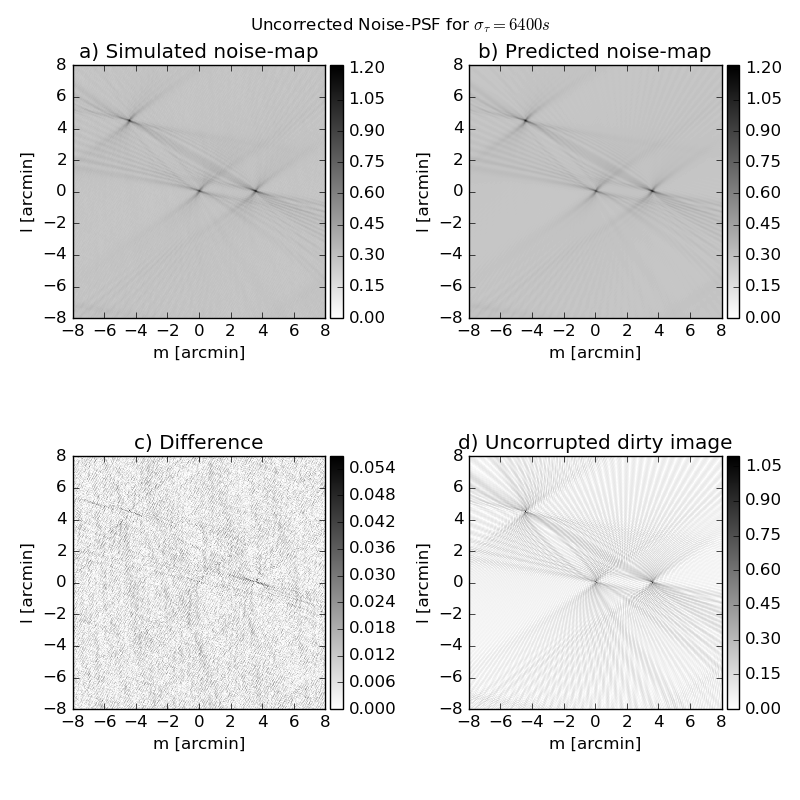
\includegraphics[width=\textwidth]{images/Ctime6400-noisePSFandDirty-uncorr.png}
\caption{\label{whatever} {Noise-map of sky with correlated gain errors and three point sources. The colourbars of (a), (b) and (c) have dimensionless units, while that of (d) is in Jansky. Note the presence of structure in the residuals (c): these show the limits of our hypothesis that sources are well-separated.}}
\end{figure}

\subsection{Quality-based Weighting Schemes}

\pg
The quality-based weighting schemes developed in this section can then be understood as ways to change the noise-distribution: one minimises the constant component of the noise-map, while the other seeks to flatten the noise-PSF. Only the first was implemented for use on real data: the other suffered from poor conditioning. This weighting scheme consists of down-weighting each visibility by an estimate of the variance of residual.
\begin{align}
w_{b} &= \frac{1}{\Var{\matGains_{b}}}
\end{align}

\begin{figure}[h!]
\begin{subfigure}{.49\textwidth}
\resizebox{\hsize}{!}{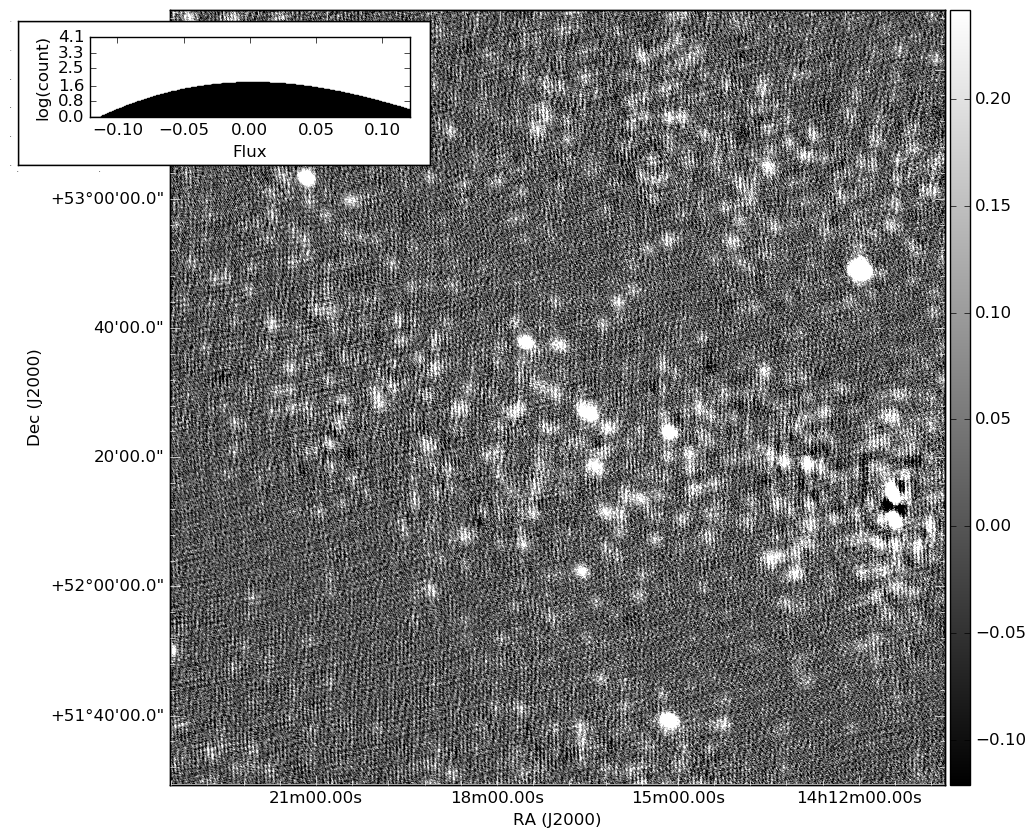
\includegraphics{images/paperfig-noweights.png}}
\caption{\label{image.3c295.nocorr1} Poorly-calibrated, unweighted restored image of the sky near the centre of the Extended Groth Strip. {Units of colourbar are Jy/bm}. rms=86.4mJy/beam}
\end{subfigure}
\begin{subfigure}{.49\textwidth}
\resizebox{\hsize}{!}{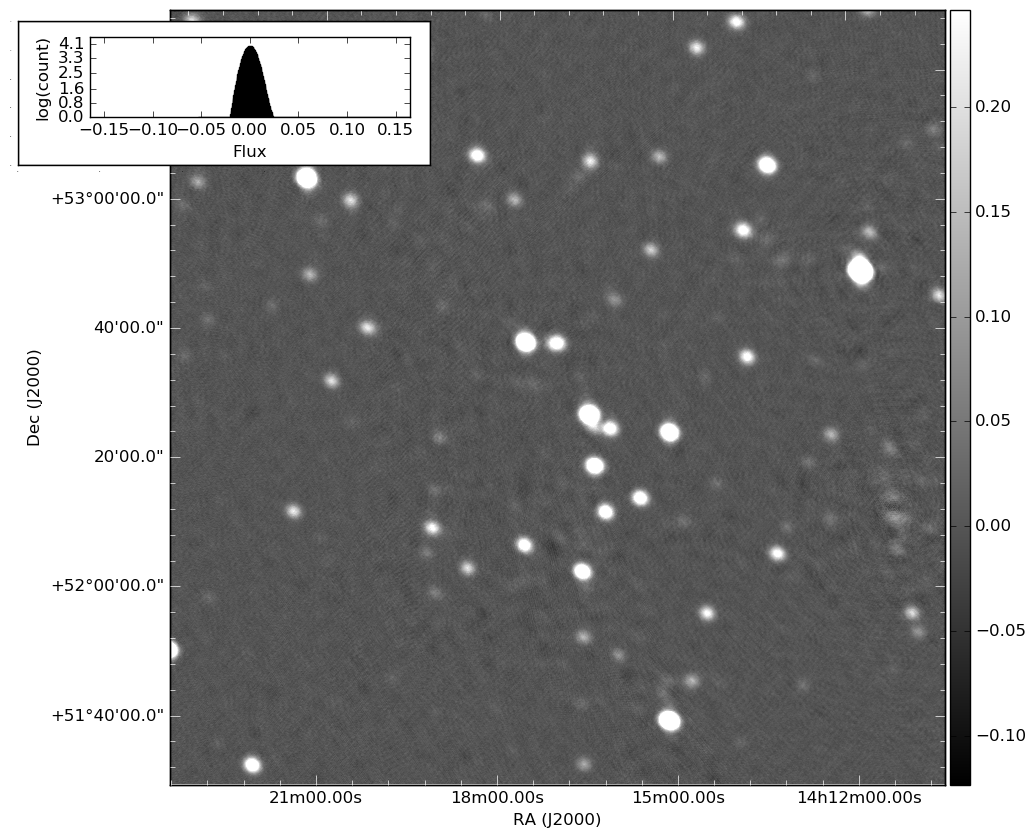
\includegraphics{images/paperfig-antweights.png}}
\caption{\label{image.3c295.antcorr1} Image made with the application of antenna-based, sensitivity-optimal weighting. Solution interval of 2 minutes, half the bandwidth. rms=6.69mJy/beam}
\end{subfigure}
\caption{\label{stuff} Copies of \cref{image.3c295.nocorr} and \cref{image.3c295.antcorr1}, used to show the impact of the weighting schemes on real data.}
\end{figure}

\pg
The cov-cov relationship is likely going to be revisited at a future time to be expanded to more complex cases. Much work nevertheless remains: in both improving the conditioning of the covariance matrix estimation, a necessary prerequisite for its successful application, and in attempting to generalise the framework to account for DDEs, more sophisticated interval solutions (e.g. convolution with a Gaussian with characteristic width equal to the solution interval rather than simple binning), and other modern features of calibration solvers. Similarly, the effect of sky model incompleteness has yet to be investigated thoroughly, and simulation work to this effect could bring great insight on this still-open question.

\pg
Similarly, the question of properly conditioning our estimates of the visibility covariance matrix remains open. This would be a potentially fertile avenue of research, as being able to estimate the full visibility covariance matrix reliably and swiftly could lead to the ability to implement ``artefact-optimal" weights: that is, attempt to completely flatten the noise-PSF, at the cost of increasing the constant, ``thermal" noise component of the image's noise-map.



\section{Imaging the Extended Groth strip}

\pg
We applied our newly-developed weighting schemes to the problem of imaging the Extended Groth Strip, a rich extragalactic field near a bright 3C source. In so doing, we followed a four-part strategy, consisting of:
\begin{itemize}
\item Imaging the full LOFAR primary beam with the core and remote stations. This requires direction-dependent calibration;
\item Creating a high-resolution, frequency-dependent model of 3C295 to use as an international station calibrator source. This required direction-independent self-calibration with a strong imaging $uv$-cut;
\item Preliminary investigation of the impact of directional gain errors from direction-independent calibration using the model of 3C295 obtained from the step above;
\item Creating a dirty map of the EGS after subtracting all sources from the widefield image \& the high-resolution model of 3C295.
\end{itemize}

\pg
Of these four points, only the first three were successfully carried out. Modeling and subtracting all the sources in the primary beam (barring 3C295) proved to be an extremely time-consuming task, and could not be completed in time. We therefore limit our discussion to the first three points, treating the last as the subject for future work.

\subsection{Imaging the LOFAR primary beam}

\subsection{Using 3C295 to self-calibrate the international stations}

\subsection{Quantifying the impact of international station directional gain errors}

\pg
For the second item, a high-resolution, frequency-dependent model of 3C295 was successfully obtained. With this model, the international LOFAR stations were calibrated well enough that other calibrator sources were visible and morphologically-interesting, even with strong Briggs weighting (optimising for resolution at the cost of signal-to-noise). Other sources in the field were visible; with the proper subtraction of 3C295 and the other sources in the field, a dirty map of the EGS would be within easy reach, and all that remains would be to deconvolve it. This is a relatively straightforward but time-consuming operation. Afterwards, the necessary checks (integrated flux, source completeness, astrometric accuracy) will need to be performed before the image is scientifically useful. 


\pg
Much work thus remains. Due to a series of setbacks and complications, only very preliminary results were obtained by the end of the doctorate's three-year period. These preliminary results are shown in this manuscript, and while they are not of science-grade quality (no astrometric corrections, proper flux bootstrapping, strategy likely needs revisiting for best results) they are nevertheless useful markers of the wealth of information available in the EGS, even with the flawed strategy used. Depending on computational resources \& work-hours available, future work could include anything from the creation of a dirty map of the EGS with the data available (which, depending on the runtime for visibility modeling, could be done in time for the defense of this thesis) to a reboot of the strategy, starting explicitly from a model including 3C295 and all other sources at low resolutions (and then improving on 3C295 at high resolutions only). It is a shame that the patchwise imaging of the EGS could not be performed by the end of the thesis, but the author hopes to be able to complete it in due time.

%
%\pg
%The algorithmic work done in this PhD was extremely fruitful, though its applications to data were less so. Much future work remains: in particular, imaging the EGS has not yet been done, due to technical \& time constraints (1 day / subband to model visibilities for out-of-field source subtraction). 